\section{Showcases}\label{appx:showcase_addition}

Figure~\ref{fig:showcases_add_01} and Figure~\ref{fig:showcases_add_02} presents more qualitative comparison showcases between the baseline STIT model and the proposed RDFR framework on the ETTh2 and ETTm1 dataset (input-96-predict-96).
In Figure~\ref{fig:showcases_add_01}, the top row (a-c) illustrates critical limitations in the baseline, including incomplete sequence generation due to early stopping, low forecasting accuracy, and severe formatting errors where missing decimal points result in extreme outliers (specifically, values like $1.25$ are erroneously output as $125$). In contrast, the bottom row (d-f) demonstrates that RDFR effectively rectifies these issues, ensuring complete prediction lengths, significantly enhanced precision, and the elimination of formatting-induced anomalies.

In Figure~\ref{fig:showcases_add_02}, the top row highlights the limitations of the baseline STIT model, which suffers from incomplete sequence generation, low accuracy, and severe formatting hallucinations. Specifically, in case (c), the model generates an erroneous space after the decimal point (e.g., splitting $-1.75$ into $-1$ and $75$), which causes the parser to misinterpret the fractional component as a massive integer outlier. The bottom row demonstrates that the proposed RDFR framework effectively rectifies these syntactic, semantic, and structural issues, ensuring continuous and robust time series prediction.

\begin{figure}[htbp]\centering
\begin{subfigure}[t]{0.32\linewidth}\centering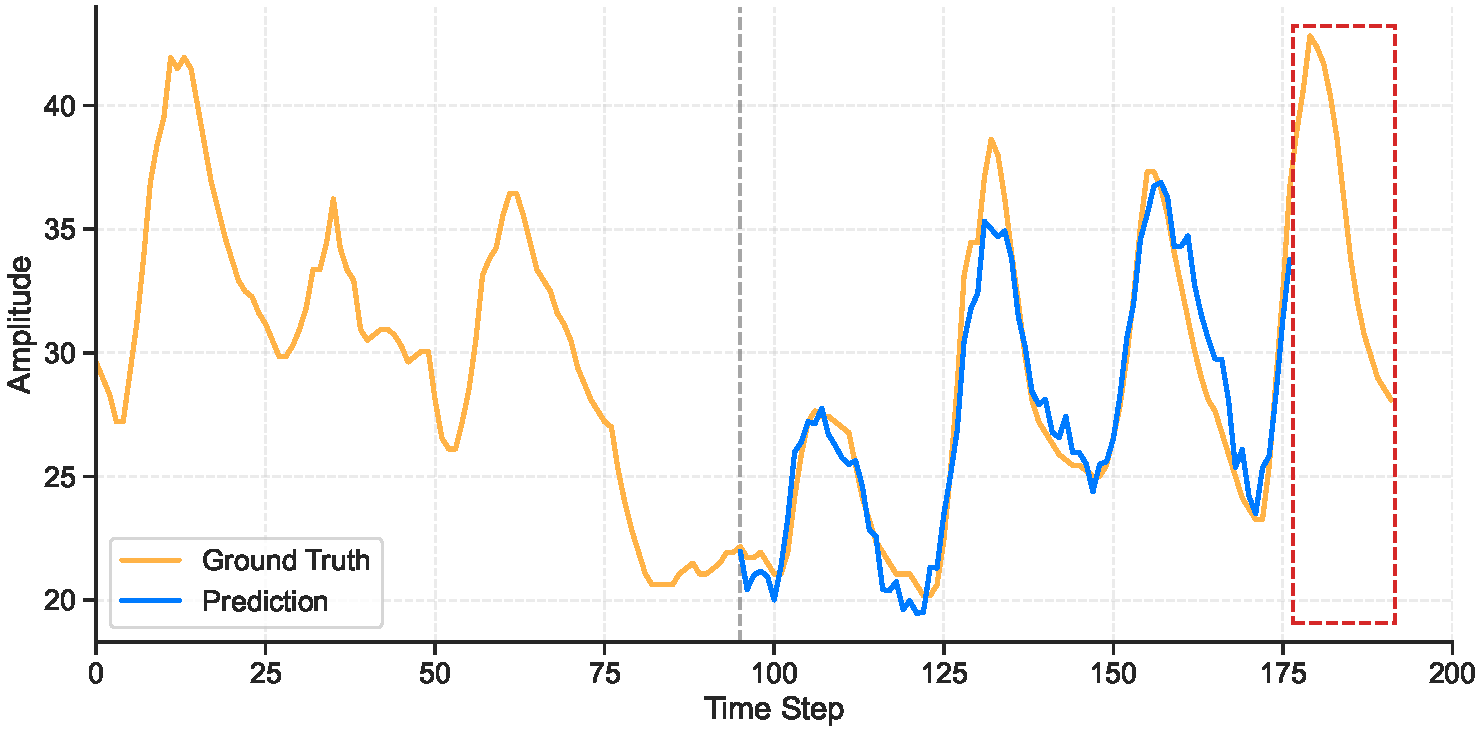
\includegraphics[width=\linewidth]{figures/appendix/showcase_additional/ground_truth_plot_01_len.pdf}\caption{Incomplete prediction (early stopping).}\label{fig:showcase01_add01-len}\end{subfigure}%
\hfill%
\begin{subfigure}[t]{0.32\linewidth}\centering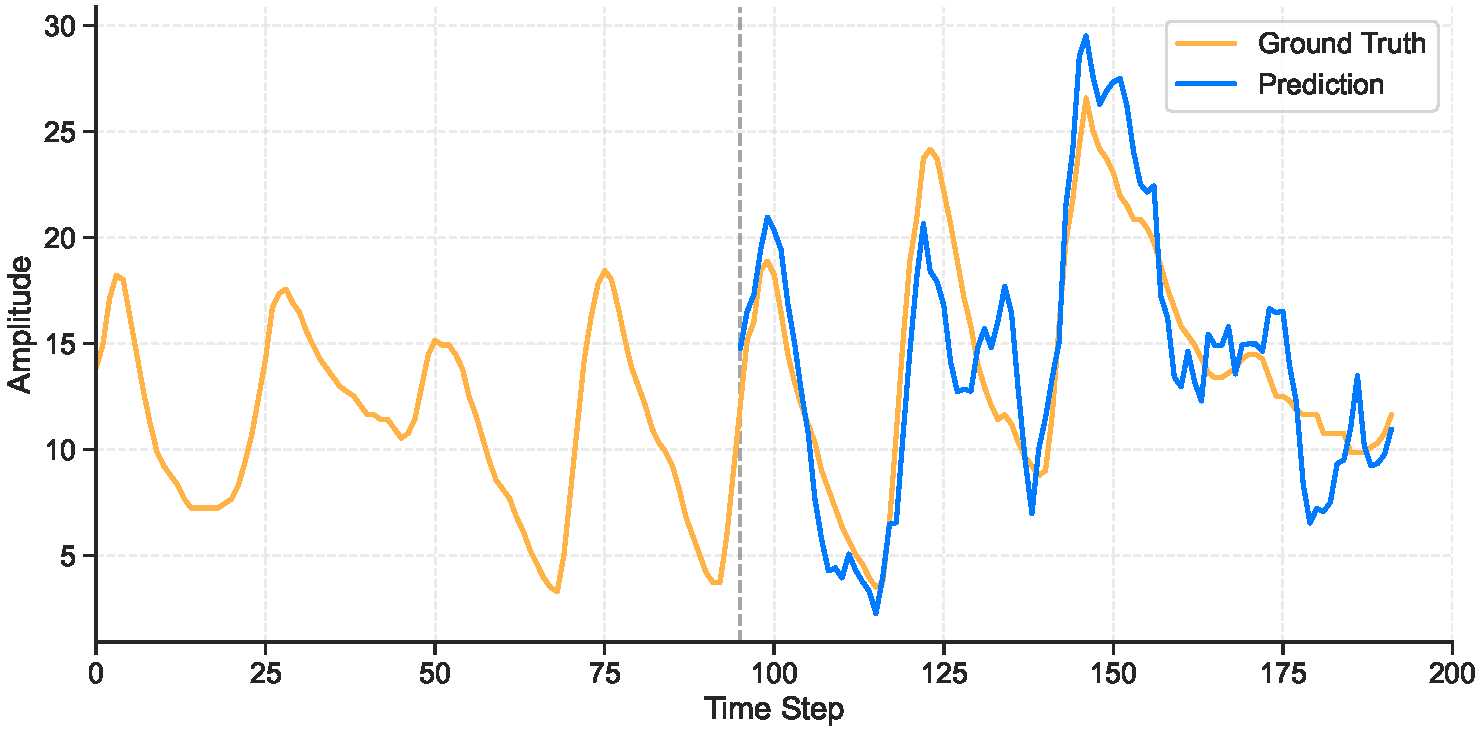
\includegraphics[width=\linewidth]{figures/appendix/showcase_additional/ground_truth_plot_02_mse.pdf}\caption{Low prediction accuracy (high MSE).}\label{fig:showcase02_add01-mse}\end{subfigure}%
\hfill%
\begin{subfigure}[t]{0.32\linewidth}\centering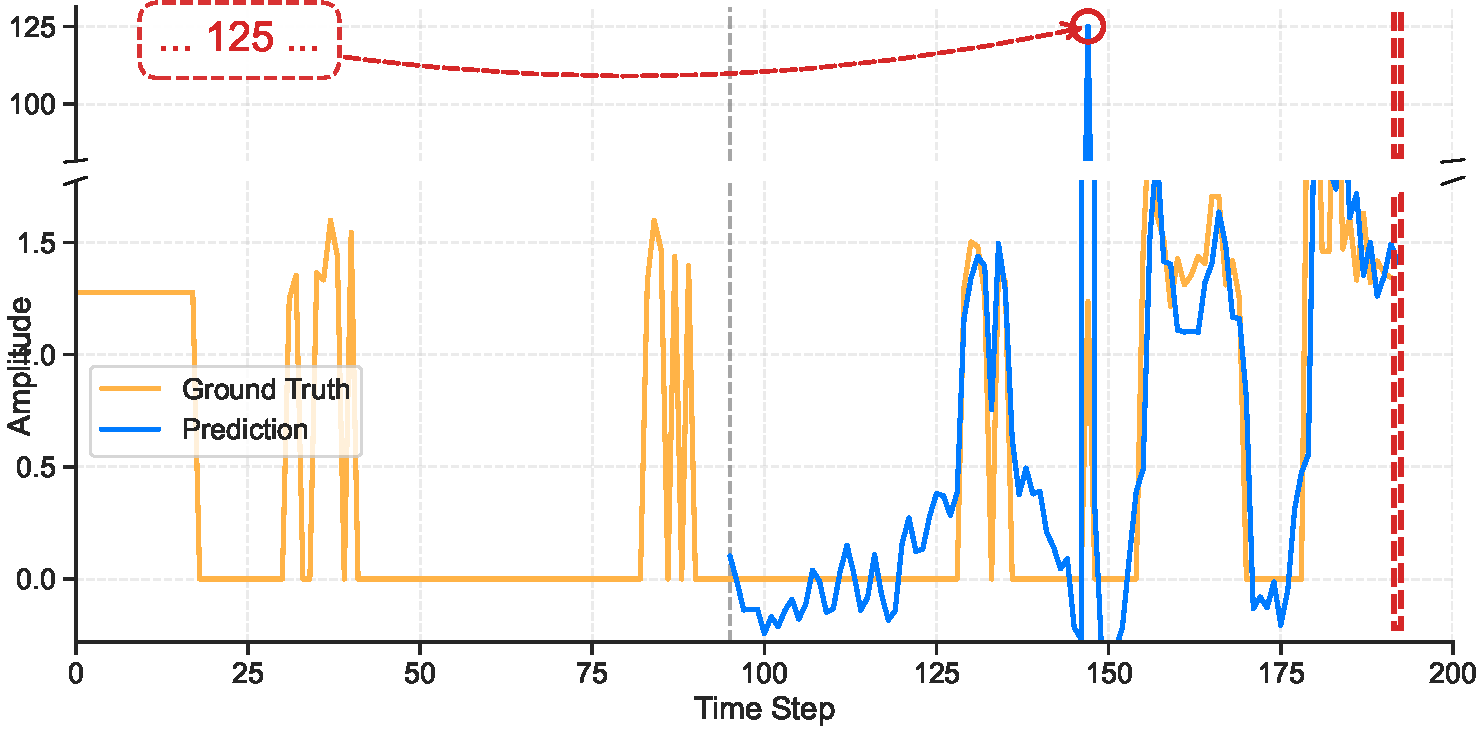
\includegraphics[width=\linewidth]{figures/appendix/showcase_additional/ground_truth_plot_03_decimal.pdf}\caption{Formatting error causing abnormal spikes.}\label{fig:showcase03_add01-fmt}\end{subfigure}%
\par\medskip
\begin{subfigure}[t]{0.32\linewidth}\centering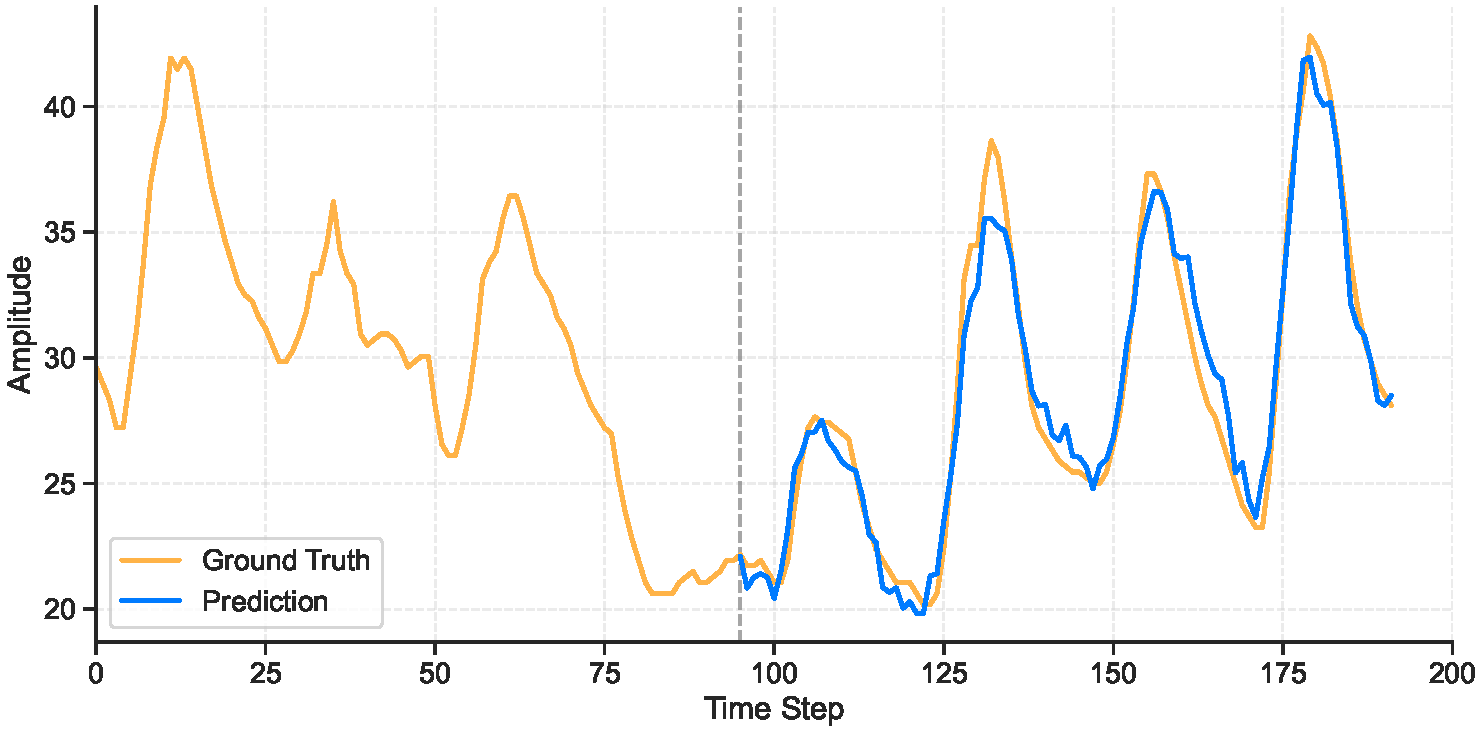
\includegraphics[width=\linewidth]{figures/appendix/showcase_additional/ground_truth_plot_01.pdf}\caption{Correction of prediction length.}\label{fig:showcase01_add01}\end{subfigure}%
\hfill%
\begin{subfigure}[t]{0.32\linewidth}\centering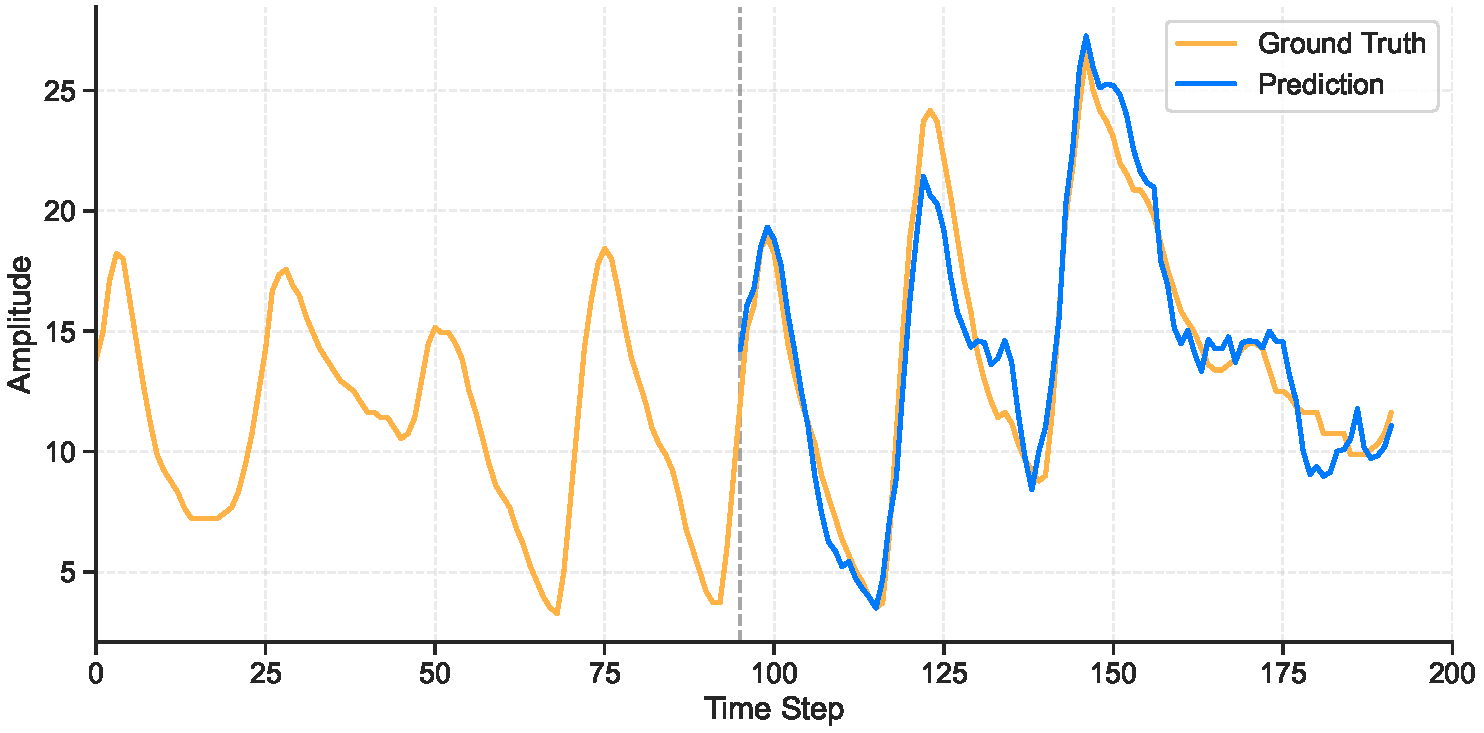
\includegraphics[width=\linewidth]{figures/appendix/showcase_additional/ground_truth_plot_02.pdf}\caption{Enhanced prediction precision.}\label{fig:showcase02_add01}\end{subfigure}%
\hfill%
\begin{subfigure}[t]{0.32\linewidth}\centering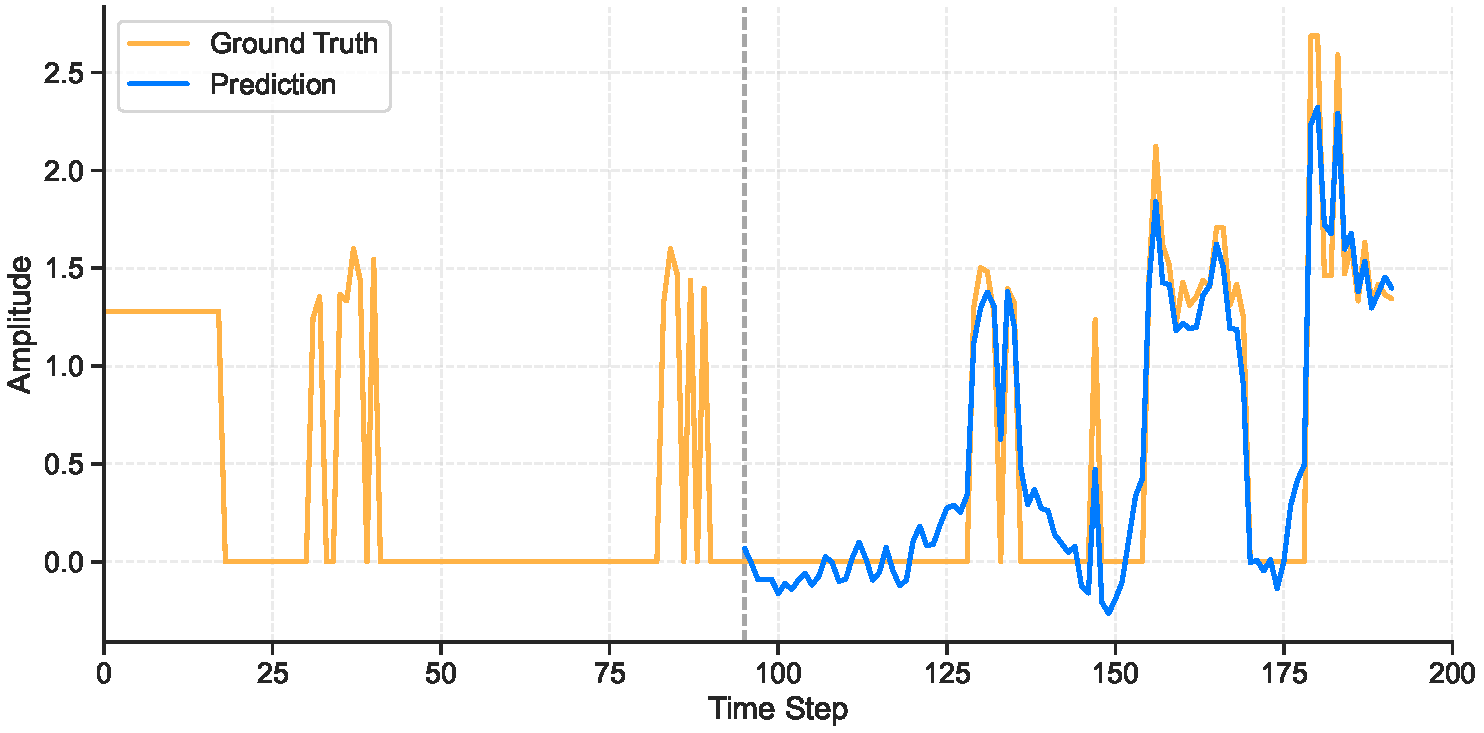
\includegraphics[width=\linewidth]{figures/appendix/showcase_additional/ground_truth_plot_03.pdf}\caption{Rectification of output format and outliers.}\label{fig:showcase03_add01}\end{subfigure}%

\caption{More showcases visualization of input-96-predict-96 results on the ETTh2 dataset. The top row (a-c) displays the baseline performance of the STIT model, which exhibits limitations in sequence length, accuracy, and output formatting. The bottom row (d-f) showcases the improvements achieved after applying the proposed RDFR framework on the corresponding samples.}\label{fig:showcases_add_01}\end{figure}


\input{figures/appendix/showcase_additional/showcase_additional_02}
